\chapter{Los elementos en el Universo y en la Tierra}\label{ch:g9:elements-universe-earth}

El calcio de tus huesos, el hierro de tu sangre y el oxígeno que
respiras no se fabricaron en la Tierra. Se fabricaron en el interior de
estrellas que nacieron y murieron antes de que naciera el Sol, y han
pasado de la roca al mar, del mar a la planta y de la planta al animal
durante miles de millones de años. Algunos elementos están por todas
partes; otros son raros. ¿Qué elementos forman las estrellas, la Tierra,
los océanos y a nosotros mismos?

\begin{recall}
Un \omterm{def:g9:inside-the-atom:element}{elemento químico} es el conjunto de los \omterm{def:g7:atoms-and-molecules:atom}{átomos} con el mismo \omterm{def:g9:inside-the-atom:atomic-number}{número
atómico} $Z$; la masa de un \omterm{def:g7:atoms-and-molecules:atom}{átomo} se acerca a
$A \times \qty{1.67e-27}{kg}$, donde $A$ es su \omterm{def:g9:inside-the-atom:atomic-number}{número másico}
(\cref{ch:g9:inside-the-atom}). La \omterm{def:g9:periodic-table-first-look:periodic-table}{tabla periódica} enumera los 118
elementos por \omterm{def:g9:inside-the-atom:atomic-number}{número atómico} (\cref{ch:g9:periodic-table-first-look}).
El \omterm{def:g4:air-a-mixture-of-gases:air}{aire} tiene unas cuatro quintas partes de nitrógeno y una quinta
parte de oxígeno (\cref{ch:g4:air-a-mixture-of-gases}).
\end{recall}

\section{Los elementos de las estrellas}

\begin{definition}[Abundancia]\label{def:g9:elements-universe-earth:abundance}
La \emph{abundancia}\index{abundancia} de un elemento en un cuerpo
material (una estrella, la corteza terrestre, el océano, un ser vivo) es
su parte de la masa total, que se suele dar en tanto por ciento.
\end{definition}

\begin{proposition}[El Sol es hidrógeno y helio]\label{prop:g9:elements-universe-earth:sun}
% ledger: ab:sun-X, ab:sun-Y, ab:sun-Z
La superficie del Sol es, en masa, alrededor de un \qty{74}{\percent}
de hidrógeno y un \qty{25}{\percent} de helio; todos los demás elementos
juntos solo suponen alrededor del \qty{1.3}{\percent}. La mayor parte de
la materia visible del Universo tiene una composición parecida:
hidrógeno y helio, con una pizca de todo lo demás.
\end{proposition}

\begin{proposition}[Elementos fabricados en las estrellas]\label{prop:g9:elements-universe-earth:stars}
El hidrógeno y la mayor parte del helio se formaron en los primeros
minutos del Universo. Casi todos los elementos más pesados (el carbono,
el oxígeno, el hierro, el oro) se fabricaron más tarde, en el interior
de las estrellas, y se dispersaron por el espacio cuando las estrellas
explotaron. De ese polvo enriquecido se formaron nuevas estrellas y
nuevos planetas. Cómo lo hacen las estrellas lo cuenta el libro de
física.
\end{proposition}

\begin{omfigure}
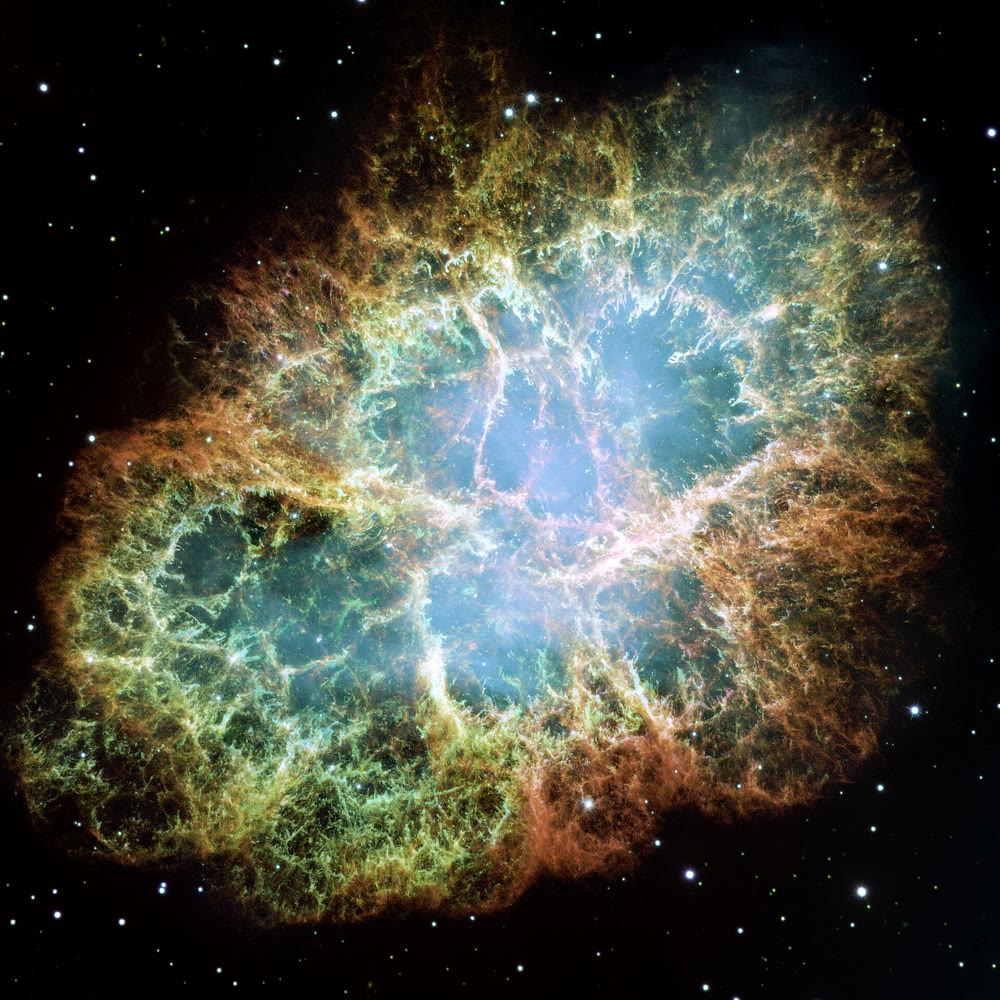
\includegraphics[width=0.45\linewidth]{images/book1/crab-nebula.jpg}

{\small La nebulosa del Cangrejo, la nube que dejó una estrella que
explotó hace casi mil años y que esparce elementos nuevos por el espacio
(NASA, ESA, J.~Hester y A.~Loll).}
\end{omfigure}

\section{La Tierra}

\begin{proposition}[La corteza terrestre]\label{prop:g9:elements-universe-earth:crust}
% ledger: ab:crust-O, ab:crust-Si, ab:crust-Al, ab:crust-Fe, ab:crust-Ca, ab:crust-Na, ab:crust-K, ab:crust-Mg, ab:crust-first10
La fina piel rocosa de la Tierra, la corteza, es casi la mitad oxígeno y
más de una cuarta parte silicio, en masa: las rocas y la arena son sobre
todo óxidos de silicio y de unos pocos \omterm{def:g9:periodic-table-first-look:metal}{metales}. Ocho elementos (el
oxígeno, el silicio, el aluminio, el hierro, el calcio, el sodio, el
potasio y el magnesio) forman alrededor del \qty{99}{\percent} de ella.
El hidrógeno y el helio, tan corrientes en las estrellas, son escasos:
los gases ligeros escaparon de la Tierra joven.
\end{proposition}

\begin{remark}[El interior de la Tierra]\label{rem:g9:elements-universe-earth:core}
La corteza no es toda la Tierra. El hierro, pesado, se hundió hacia el
centro cuando la Tierra joven estaba fundida: el \omterm{def:g9:inside-the-atom:nucleus}{núcleo} de la Tierra es
sobre todo hierro, con algo de níquel.
\end{remark}

\begin{proposition}[Los océanos y el aire]\label{prop:g9:elements-universe-earth:ocean}
% ledger: sea:salts-share, sea:NaCl-ions, sea:MgSO4-ions, air:N2, air:O2
El agua del mar es sobre todo agua (hidrógeno y oxígeno) con alrededor
de un \qty{3.5}{\percent} de sales disueltas, en masa. Entre los \omterm{def:g9:ions:ion}{iones}
disueltos, el cloruro y el sodio suponen alrededor del \qty{85}{\percent},
y el magnesio y el sulfato, otro \qty{10}{\percent}. El \omterm{def:g4:air-a-mixture-of-gases:air}{aire} es sobre
todo nitrógeno y oxígeno.
\end{proposition}

\begin{omfigure}
\begin{tikzpicture}
\begin{axis}[xbar, width=0.40\linewidth, height=5.4cm, xmin=0, xmax=85,
    bar width=7pt, symbolic y coords={Mg,K,Na,Ca,Fe,Al,Si,O}, ytick=data,
    xlabel={tanto por ciento de la masa}, title={\small la corteza terrestre},
    nodes near coords, nodes near coords style={font=\scriptsize},
    tick label style={font=\small}, label style={font=\small},
    axis lines*=left, enlarge y limits=0.08]
% ledger: ab:crust-O, ab:crust-Si, ab:crust-Al, ab:crust-Fe, ab:crust-Ca, ab:crust-Na, ab:crust-K, ab:crust-Mg
\addplot[fill=omDef!45, draw=omDef] coordinates {(46.6,O) (27.7,Si) (8.1,Al)
  (5.0,Fe) (3.6,Ca) (2.8,Na) (2.6,K) (2.1,Mg)};
\end{axis}
\end{tikzpicture}\hfill
\begin{tikzpicture}
\begin{axis}[xbar, width=0.40\linewidth, height=5.4cm, xmin=0, xmax=85,
    bar width=7pt, symbolic y coords={{P},{N},{Ca},{H},{C},{O}}, ytick=data,
    xlabel={tanto por ciento de la masa}, title={\small un cuerpo humano},
    nodes near coords, nodes near coords style={font=\scriptsize},
    tick label style={font=\small}, label style={font=\small},
    axis lines*=left, enlarge y limits=0.1]
% ledger: body:atoms-O, body:atoms-C, body:atoms-H, body:atoms-N, body:atoms-Ca, body:atoms-P (masses = atoms x atomic mass, over 70 kg)
\addplot[fill=omProp!45, draw=omProp] coordinates {(61.1,O) (22.9,C) (10.1,H)
  (1.3,N) (1.5,Ca) (0.7,P)};
\end{axis}
\end{tikzpicture}

{\small \omterm{def:g9:elements-universe-earth:abundance}{Abundancias} en masa. A la izquierda, los ocho elementos
principales de la corteza terrestre. A la derecha, los seis elementos
principales del cuerpo de un adulto delgado (calculados a partir del
número estimado de \omterm{def:g7:atoms-and-molecules:atom}{átomos}).}
\end{omfigure}

\section{El cuerpo humano}

\begin{proposition}[De qué estamos hechos]\label{prop:g9:elements-universe-earth:body}
% ledger: body:atoms-O, body:atoms-C, body:atoms-H, body:atoms-N, body:atoms-Ca, body:atoms-P, body:atoms-total
En masa, el cuerpo de un adulto delgado es alrededor de un
\qty{61}{\percent} de oxígeno, un \qty{23}{\percent} de carbono y un
\qty{10}{\percent} de hidrógeno (sobre todo en el agua y en las
\omterm{def:g7:atoms-and-molecules:molecule}{moléculas} de la vida), seguidos del nitrógeno, el calcio (en los huesos
y los dientes) y el fósforo. Si se cuentan \omterm{def:g7:atoms-and-molecules:atom}{átomos} en lugar de masa, el
orden cambia: en un cuerpo hay más \omterm{def:g7:atoms-and-molecules:atom}{átomos} de hidrógeno que todos los
demás \omterm{def:g7:atoms-and-molecules:atom}{átomos} juntos, porque los \omterm{def:g7:atoms-and-molecules:atom}{átomos} de hidrógeno son muy ligeros. Un
cuerpo de \qty{70}{kg} contiene alrededor de $7 \times 10^{27}$ \omterm{def:g7:atoms-and-molecules:atom}{átomos}.
\end{proposition}

\begin{method}[Leer un gráfico de abundancias]\label{met:g9:elements-universe-earth:read}
\begin{enumerate}
  \item Comprobar qué se mide: la masa (en la mayoría de los gráficos) o
        el número de \omterm{def:g7:atoms-and-molecules:atom}{átomos}.
  \item Leer la parte de cada elemento; sumar las de los principales
        para ver cuánto abarcan.
  \item Para comparar dos cuerpos, buscar los elementos comunes a los
        dos y los que solo están en uno.
\end{enumerate}
El oxígeno encabeza los dos gráficos de este capítulo: es el elemento
más abundante en masa de la corteza y del cuerpo humano.
\end{method}

\section{Los mismos átomos, reciclados}

\begin{example}[El viaje de un átomo de carbono]\label{ex:g9:elements-universe-earth:journey}
Un \omterm{def:g7:atoms-and-molecules:atom}{átomo} de carbono fabricado hace mucho tiempo en una estrella puede
pasar millones de años en una caliza, ser liberado como dióxido de
carbono por un volcán, ser captado por una hoja, formar parte de un
azúcar en una fruta, pasar a un animal que se come la fruta y volver a
ser espirado como dióxido de carbono. Los \omterm{def:g5:irreversible-changes:chemical-change}{cambios químicos} no destruyen
los \omterm{def:g7:atoms-and-molecules:atom}{átomos}: los van pasando de unos a otros.
\end{example}

\begin{omfigure}
\begin{tikzpicture}[font=\small,
    box/.style={draw=omDef, fill=omDef!6, rounded corners=2pt, align=center,
      minimum height=0.85cm, text width=2.3cm}]
  \node[box] (a) at (0,2.2) {en una roca\\ (caliza)};
  \node[box] (b) at (4.3,2.2) {en el aire\\ (\ce{CO2})};
  \node[box] (c) at (8.6,2.2) {en una hoja\\ (azúcar)};
  \node[box] (d) at (8.6,0) {en un animal};
  \node[box] (e) at (4.3,0) {espirado\\ (\ce{CO2})};
  \draw[->, thick, omProp] (a) -- node[above, font=\footnotesize] {volcán} (b);
  \draw[->, thick, omProp] (b) -- (c);
  \draw[->, thick, omProp] (c) -- node[right, font=\footnotesize] {comido} (d);
  \draw[->, thick, omProp] (d) -- (e);
  \draw[->, thick, omProp] (e) -- (b);
\end{tikzpicture}

{\small Un \omterm{def:g7:atoms-and-molecules:atom}{átomo} de carbono pasa de la roca al \omterm{def:g4:air-a-mixture-of-gases:air}{aire}, del \omterm{def:g4:air-a-mixture-of-gases:air}{aire} a la hoja,
de la hoja al animal y vuelve al \omterm{def:g4:air-a-mixture-of-gases:air}{aire}: el \omterm{def:g7:atoms-and-molecules:atom}{átomo} mismo nunca se destruye.}
\end{omfigure}

\begin{omfigure}
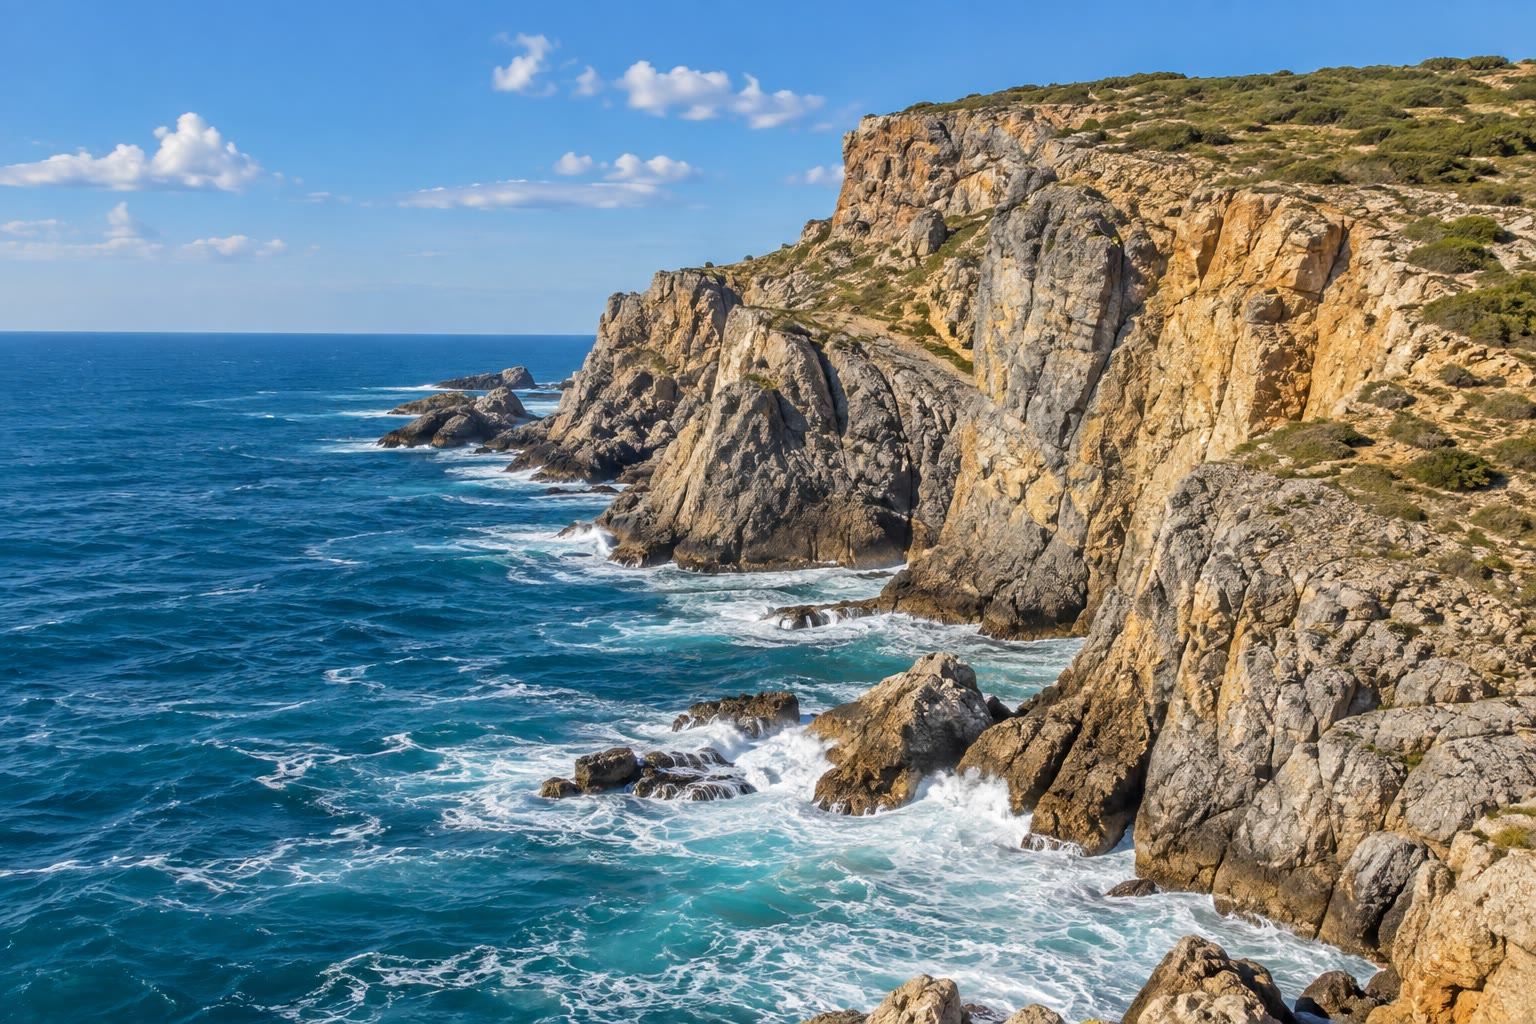
\includegraphics[width=0.55\linewidth]{images/book1/ai/g9-coastal-cliff.jpg}

{\small Roca, mar y \omterm{def:g4:air-a-mixture-of-gases:air}{aire}: tres \omterm{def:g6:pure-substances-and-mixtures:mixture}{mezclas} muy distintas de los mismos
elementos.}
\end{omfigure}

\section{Ejercicios}

\begin{exercise}[$\star$]\label{exo:g9:elements-universe-earth:1}
¿Qué dos elementos forman casi todo el Sol?
\end{exercise}

\begin{exercise}[$\star$]\label{exo:g9:elements-universe-earth:2}
¿Qué elemento es el más abundante en la corteza terrestre? ¿Y en el
cuerpo humano (en masa)?
\end{exercise}

\begin{exercise}[$\star$]\label{exo:g9:elements-universe-earth:3}
¿Dónde se fabricaron la mayoría de los elementos más pesados que el
helio?
\end{exercise}

\begin{exercise}[$\star$]\label{exo:g9:elements-universe-earth:4}
¿Qué porcentaje de la masa del agua del mar es sal disuelta?
\end{exercise}

\begin{exercise}[$\star\star$]\label{exo:g9:elements-universe-earth:5}
Con el gráfico de la corteza, suma las partes del oxígeno y del
silicio. ¿Qué fracción de la corteza es eso, más o menos?
\end{exercise}

\begin{exercise}[$\star\star$]\label{exo:g9:elements-universe-earth:6}
¿Por qué hay tan poco hidrógeno y tan poco helio en la corteza
terrestre, si el Sol está hecho casi por completo de ellos?
\end{exercise}

\begin{exercise}[$\star\star$]\label{exo:g9:elements-universe-earth:7}
¿Qué masa de carbono hay en un cuerpo de \qty{70}{kg} que tiene un
\qty{23}{\percent} de carbono?
\end{exercise}

\begin{exercise}[$\star\star$]\label{exo:g9:elements-universe-earth:8}
¿Por qué el oxígeno es el elemento más abundante del cuerpo en masa,
mientras que el hidrógeno es el más abundante en número de \omterm{def:g7:atoms-and-molecules:atom}{átomos}?
\end{exercise}

\begin{exercise}[$\star\star$]\label{exo:g9:elements-universe-earth:9}
Un bloque de granito de \qty{1000}{kg} es un trozo típico de la corteza.
Con el gráfico, ¿qué masa de aluminio contiene, más o menos?
\end{exercise}

\begin{exercise}[$\star\star$]\label{exo:g9:elements-universe-earth:10}
¿Qué elementos aparecen a la vez entre los elementos principales de la
corteza y entre los del cuerpo humano?
\end{exercise}

\begin{exercise}[$\star\star\star$]\label{exo:g9:elements-universe-earth:11}
Un cuerpo de \qty{70}{kg} contiene alrededor de \qty{1.06}{kg} de
calcio. Calcula la masa de un \omterm{def:g7:atoms-and-molecules:atom}{átomo} de calcio ($A = 40$) y, después, el
número de \omterm{def:g7:atoms-and-molecules:atom}{átomos} de calcio. Escríbelo en notación científica.
\end{exercise}

\begin{exercise}[$\star\star\star$]\label{exo:g9:elements-universe-earth:12}
Todos los \omterm{def:g7:atoms-and-molecules:atom}{átomos} de tu cuerpo han formado parte antes de otras cosas.
Usa el viaje de un \omterm{def:g7:atoms-and-molecules:atom}{átomo} de carbono para explicar por qué el número
total de \omterm{def:g7:atoms-and-molecules:atom}{átomos} de carbono de la Tierra apenas cambia.
\end{exercise}

\section{Problema: ¿Cuántos átomos soy?}

\begin{problem}[{Problema de fin de semana --- de un gráfico de
abundancias al número de átomos de oxígeno de un cuerpo humano}]
\label{pb:g9:elements-universe-earth:1}
% ledger: body:atoms-O, body:atoms-total
Un adulto delgado de \qty{70}{kg} es, en masa, alrededor de un
\qty{61}{\percent} de oxígeno, un \qty{23}{\percent} de carbono y un
\qty{10}{\percent} de hidrógeno. Toma como masa de un \omterm{def:g9:inside-the-atom:proton}{nucleón}
\qty{1.67e-27}{kg}; un \omterm{def:g7:atoms-and-molecules:atom}{átomo} de oxígeno tiene 16 \omterm{def:g9:inside-the-atom:proton}{nucleones}, uno de
carbono 12 y uno de hidrógeno 1. Se desprecian los \omterm{def:g9:inside-the-atom:nucleus}{electrones}.

\medskip
\noindent\textbf{Parte I --- Las masas.}
\begin{enumerate}
  \item Calcula la masa de oxígeno del cuerpo.
  \item Calcula la masa de carbono y la de hidrógeno.
  \item ¿Qué porcentaje de la masa forman juntos estos tres elementos?
  \item La mayor parte de este oxígeno y de este hidrógeno está en un
        solo compuesto. ¿Cuál?
\end{enumerate}

\medskip
\noindent\textbf{Parte II --- Un \omterm{def:g7:atoms-and-molecules:atom}{átomo}.}
\begin{enumerate}[resume]
  \item Calcula la masa de un \omterm{def:g7:atoms-and-molecules:atom}{átomo} de oxígeno.
  \item Calcula la masa de un \omterm{def:g7:atoms-and-molecules:atom}{átomo} de carbono y la de un \omterm{def:g7:atoms-and-molecules:atom}{átomo} de
        hidrógeno.
  \item ¿Cuántos \omterm{def:g7:atoms-and-molecules:atom}{átomos} de hidrógeno pesan lo mismo que un \omterm{def:g7:atoms-and-molecules:atom}{átomo} de
        oxígeno?
  \item ¿Por qué se pueden despreciar los \omterm{def:g9:inside-the-atom:nucleus}{electrones}?
\end{enumerate}

\medskip
\noindent\textbf{Parte III --- El recuento.}
\begin{enumerate}[resume]
  \item Calcula el número de \omterm{def:g7:atoms-and-molecules:atom}{átomos} de hidrógeno del cuerpo.
  \item Calcula el número de \omterm{def:g7:atoms-and-molecules:atom}{átomos} de carbono.
  \item Calcula el número de \omterm{def:g7:atoms-and-molecules:atom}{átomos} de oxígeno del cuerpo.
  \item Una estimación cuidadosa da $1.61 \times 10^{27}$ \omterm{def:g7:atoms-and-molecules:atom}{átomos} de
        oxígeno en un cuerpo así. Compárala con tu recuento, y da el
        número de \omterm{def:g7:atoms-and-molecules:atom}{átomos} de oxígeno de un cuerpo de \qty{70}{kg} con dos
        cifras significativas.
\end{enumerate}
\end{problem}
